\chapter{Implementación de un Generador Multilenguaje}
\label{chap:implementacion de un generador }
La implementación de un Generador Multilenguaje se puede dividir en dos etapas fundamentales. Primero, se debe diseñar e implementar el DSL, y luego definir cómo se llevará a cabo la generación de código de cada elemento del dominio en los lenguajes de salida.

A su vez, estas dos etapas se pueden desglosar en un conjunto de pasos lógicos, descritos a continuación:
\begin{enumerate}
	\item Determinar el dominio que se quiere representar en el DSL.
	\item Identificar los elementos que se desean representar en el DSL.
	\item \label{item:diseñar-dsl} Dise\~nar el lenguaje del DSL.
	\item \label{item:jerarquia-de-clases}Implementar una jerarqu\'ia de clases que permita representar cada uno de los elementos del DSL como nodos de un AST.
	\item \label{item:paso-parser-lexer} Construir el analizador lexicogr\'afico y el sint\'actico.
	\item 	\label{item:generacion-de-codigo}Implementar la generaci\'on de c\'odigo de cada uno de los nodos del AST, en cada uno de los lenguajes de salida.
\end{enumerate}

En las siguientes secciones de este capítulo, se ilustran estos pasos a partir de la creación de un Generador Multilenguaje muy simple, cuyo dominio es el trabajo con operaciones aritméticas. A este Generador Multilenguaje se le llamará BASAR (del inglés Basic Arithmetic Operations).

\section{BASAR}

BASAR es un Generador Multilenguaje donde se pueden escribir expresiones aritméticas básicas, que contengan variables y asignaciones a las mismas. Con BASAR se pueden escribir expresiones como:

\begin{verbatim}
                    X = 5 + Y * 2 
\end{verbatim}
Cuando se genere su código a C\#, R, y a Common Lisp se obtendría, respectivamente:
\begin{verbatim}
                    X = 5 + Y * 2;
                    
                    X <- 5 + Y * 2
                    
                    (setf X (+ 5 (* Y 2)))
\end{verbatim}

Una vez que se tiene bien definido el dominio que se quiere representar, el siguiente paso para la construcción de un Generador Multilenguaje es identificar qué elementos del dominio deben ser incluídos.

\section{Dominio}

En el caso de BASAR, los elementos que se desean incluir son: 
\begin{itemize}
\item Suma
\item Multiplicación
\item Asignación a variable
\item Referencia a variable
\item Imprimir
\end{itemize}
Definidos estos elementos, en el siguiente paso se diseña un lenguaje que permita expresar los elementos del dominio.
\section{Lenguaje}
En este paso resulta necesario definir cómo se representa en el DSL cada uno de los elementos del dominio que se quieren incluir. En el caso de BASAR, cada elemento se pudiera representar como se muestra a continuación:
\begin{itemize}
\item   Suma: Será una función \texttt{SUMA} que posee dos parámetros.\\ 
Ejemplo: \texttt{SUMA(A,B)} 
\item   Multiplicación: operador infijo \texttt{*}.\\ Ejemplo: \texttt{A*B}
\item Asignación a variable: operador \texttt{:=}.\\
 Ejemplo: \texttt{A := B}
\item Referencia a variable: nombre de la variable.\\
 Ejemplo: \texttt{A}
\item Imprimir: función Print.\\ 
Ejemplo: \texttt{Print A}
\end{itemize}
Con este diseño del lenguaje, la expresión $X = 5 + Y * 2$ se escribiría: 
\begin{verbatim}
                    X := SUMA(5, Y*2) 
\end{verbatim}
En el caso de \gagm, los DSLs se van a diseñar como lenguajes internos en Common Lisp, por lo que la sintaxis siempre será la misma: todos los elementos se representarían como:

\begin{verbatim}
            (name-funtion arg1, arg2,..., argN).
\end{verbatim}
En este caso solo habría que definir qué nombre tendrá la función que representa a cada uno de los elementos del dominio, de forma que si la asignación se representa por la función \texttt{assign-to}, y la suma y el producto por los operadores \texttt{+}, y \texttt{*}, la expresión $X = 5 + Y * 2$ se representaría como:

\begin{verbatim}
                    (assign-to X (+ 5 (* Y 2))
\end{verbatim}
De esta forma se termina de definir el lenguaje. El siguiente paso es representar cualquier cadena del lenguaje en un AST, lo que se ejemplifica en la próxima sección.

\section{Nodos del Árbol de Sintaxis Abstracta}

Una vez diseñado el lenguaje para un Generador Multilenguaje, se debe crear una jerarquía de clases para los nodos del AST, que dependa de las especificidades del problema. En el caso de BASAR, se define  una clase por cada operación que se desea representar. Además se crea la clase \texttt{binary-operator}, de la que heredan \texttt{sum-node} y \texttt{mult-node}. En la figura \ref{nodos-para-Basar} se muestra la jerarquía de clases para este problema, y en la figura \ref{AST3}, se muestra el AST para el ejemplo de la sección anterior.
\begin{figure}
    \centering
    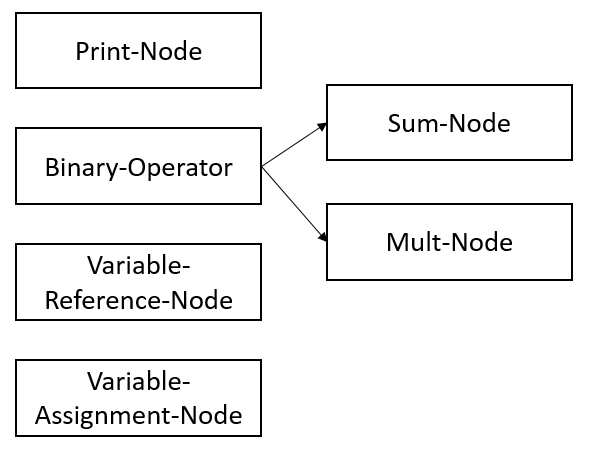
\includegraphics[width=0.5\textwidth]{simple-jerarquia.png}
    \caption{Jeraquía de nodos del AST para BASAR}
    \label{nodos-para-Basar}
\end{figure}
\begin{figure}
    \centering
    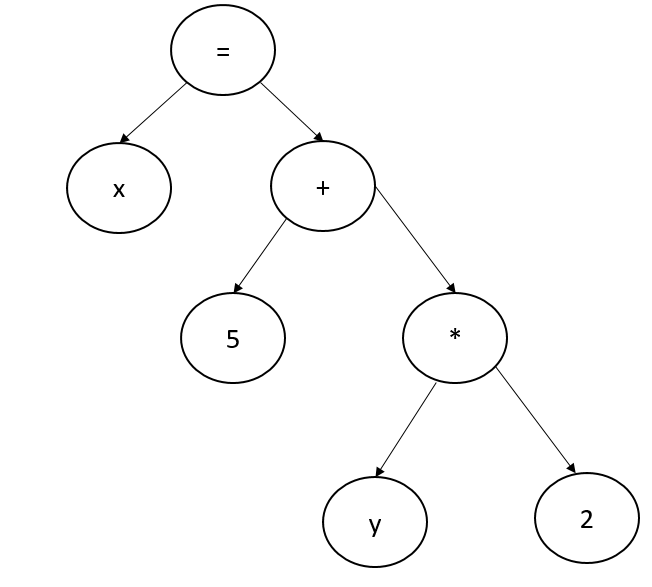
\includegraphics[width=0.5\textwidth]{AST3.png}
    \caption{AST correspondiente a la expresión: (ASSIGN-TO X (+ 5 (* Y 2))}
    \label{AST3}
  \end{figure}

  En dependencia del lenguaje de programación en el que se desee implementar un Generador Multilenguaje, puede ser necesario implementar el analizador lexicográfico y el sintáctico, para construir el AST, a partir de las cadenas del DSL. Como en {\gagm} los lenguajes para los DSLs tendrán la misma sintaxis \texttt{(nombre arg1, arg2, ..., argN)} y los ASTs se pueden obtener mediante funciones constructoras, el intérprete de Common Lisp realizará estos análisis.
  
  Terminada la construcción del AST, se procede a generar el código de sus nodos a los lenguajes de salida.
  
  \section{Generación de código }
  
Para generar el código de programas escritos en BASAR en cualquiera de los lenguajes de salida, basta con especificar cómo se escribe cada nodo del AST en el lenguaje deseado. De esta forma, para escribir el código de un programa completo se recorre el AST que lo representa, generando el código de cada nodo.

Por ejemplo, para escribir en C\# el código correspondiente al AST ilustrado en la figura \ref{AST3}, se necesita especificar cómo generar el código de cada uno de los nodos. Si \texttt{G(X)} representa la generación de código del elemento \texttt{X} se tiene que:

\begin{itemize}
    \item La asignación en C\# es: 
          \begin{verbatim}
             G(parte-izq) = G(parte-der)  
          \end{verbatim}
    \item La suma en C\# es:
     \begin{verbatim}
             G(parte-izq) + G(parte-der)  
     \end{verbatim}
    \item La multiplicación en C\# es:
       \begin{verbatim}
              G(parte-izq) * G(parte-der)  
       \end{verbatim}
    
    \item   La referencia a variable en C\# es:
       \begin{verbatim}
               Nombre-de-la-variable
       \end{verbatim}

    \item Imprimir un elemento en C\#:
     \begin{verbatim}
              Console.WriteLine(G(A))
     \end{verbatim}
    
\end{itemize}  

Una vez definida la generación de código para cada nodo y para cada lenguaje, se puede recorrer el AST generando el código. Los resultados de generar el código del AST ilustrado en \ref{AST3} en C\# y en Common Lisp serían:
\begin{verbatim}
               X = 5 + Y * 2
               
               (setf x (+ 5 (* (Y 2))))
\end{verbatim}

Una de las características principales de un Generador Multilenguaje es que permite definir con facilidad nuevos lenguajes de salida. Por ejemplo, una vez definido el DSL y la generación de código hacia C\#, si se quiere incluir Common Lisp como un lenguaje de salida, solo habría que definir cómo se escribe cada nodo del AST en este nuevo lenguaje.  Si se quisiera hacer la generación de código para otro lenguaje que posea elementos comunes con C\# o Common Lisp, se puede reutilizar la generación de código que ya existe. 

%Common Lisp, puesto que el lenguaje ya está definido. 

Los pasos presentados para desarrollar la implementación de un Generador Multilenguaje serán aplicados en el próximo capítulo, cuando se presente  la herramienta \gagm, que permite agilizar estos pasos.

%Además, dichos pasos también se pueden observar en la implementación de ADOL*.  Independientemente de cual sea su dominio, esta metodología es común para el desarrollo de todos los Generadores Multilenguajes, salvo el caso de identificar los elementos del dominio a representar en su DSL.
 
% En el siguiente capítulo, se aterriza esta metodología para implementar un Generador Multilenguaje en Common Lisp y se identifican fragmentos de código repetidos que serán eliminados utilizando la herramienta propuesta en este trabajo de diploma. Además, se presenta dicha herramienta. 



%%% Local Variables:
%%% mode: latex
%%% TeX-master: "../Thesis"
%%% End:
